\documentclass{article}
\usepackage[utf8]{inputenc}
\usepackage[T1]{fontenc}
\usepackage{amsmath}
\usepackage{amssymb}
\usepackage{pgfplots}
\usepackage{tikz}
\usetikzlibrary{shapes.geometric,decorations.pathmorphing}

\begin{document}

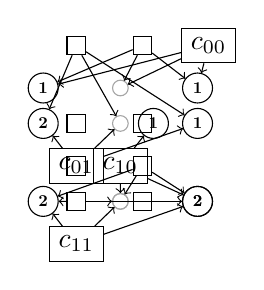
\begin{tikzpicture}[xscale=1.4,yscale=0.9]
	\node [draw,circle,scale=0.6] (v0) at (-1.5,0) {\textbf{1}};
	\node [draw,circle,scale=0.6,gray!70] (v1) at (-0.8,0) {};
	\node [draw,circle,scale=0.6] (v2) at (-0.1,0) {\textbf{1}};
	\node [draw] (c00) at (0,0.6) {$c_{00}$};
	\draw[->] (c00) -- (v0);
	\draw[->] (c00) -- (v1);
	\draw[->] (c00) -- (v2);
	
	\node [draw,circle,scale=0.6] (v0') at (-1.5,-0.5) {\textbf{2}};
	\node [draw,circle,scale=0.6,gray!70] (v1') at (-0.8,-0.5) {};
	\node [draw,circle,scale=0.6] (v2') at (-0.1,-0.5) {\textbf{1}};
	\node [draw] (c01) at (-1.2,-1.1) {$c_{01}$};
	\draw[->] (c01) -- (v0');
	\draw[->] (c01) -- (v1');
	\draw[->] (c01) -- (v2');
	
	\node [draw,circle,scale=0.6] (v0'') at (-0.5,-0.5) {\textbf{1}};
	\node [draw,circle,scale=0.6,gray!70] (v1'') at (-0.8,-1.6) {};
	\node [draw,circle,scale=0.6] (v2'') at (-0.1,-1.6) {\textbf{2}};
	\node [draw] (c10) at (-0.8,-1.1) {$c_{10}$};
	\draw[->] (c10) -- (v0'');
	\draw[->] (c10) -- (v1'');
	\draw[->] (c10) -- (v2'');
	
	\node [draw,circle,scale=0.6] (v0''') at (-1.5,-1.6) {\textbf{2}};
	\node [draw,circle,scale=0.6,gray!70] (v1''') at (-0.8,-1.6) {};
	\node [draw,circle,scale=0.6] (v2''') at (-0.1,-1.6) {\textbf{2}};
	\node [draw] (c11) at (-1.2,-2.2) {$c_{11}$};
	\draw[->] (c11) -- (v0''');
	\draw[->] (c11) -- (v1''');
	\draw[->] (c11) -- (v2''');


	\node [draw] (c00') at (-0.6,0.6) {};
	\node [draw] (c01') at (-1.2,-0.5) {};
	\node [draw] (c10') at (-0.6,-1.1) {};
	\node [draw] (c11') at (-1.2,-1.6) {};
	\node [draw] (c00'') at (-1.2,0.6) {};
	\node [draw] (c01'') at (-0.6,-0.5) {};
	\node [draw] (c10'') at (-1.2,-1.1) {};
	\node [draw] (c11'') at (-0.6,-1.6) {};

	\draw[->] (c00') -- (v0);
	\draw[->] (c00') -- (v1);
	\draw[->] (c00') -- (v2);
	\draw[->] (c00'') -- (v0');
	\draw[->] (c00'') -- (v1');
	\draw[->] (c00'') -- (v2');
	\draw[->] (c10') -- (v0''');
	\draw[->] (c10') -- (v1''');
	\draw[->] (c10') -- (v2''');
	\draw[->] (c11') -- (v0''');
	\draw[->] (c11') -- (v1''');
	\draw[->] (c11') -- (v2''');

	\end{tikzpicture}
\end{document}